% =========================================================================
% Beyond Top-K: A Typed Operator Suite for Answer-Geometry Mismatches in KGQA
%
% Draft v12.1 (2026-06-01) -- v12 reframed around answer-geometry mismatch
% and operator-driven gain (advice-driven revision over v11); v12.1 merges
% Limitations / Future Work / Appendix robustness from v5_revised.
% Full v10 manuscript: strategy_routed_graphrag_full.tex
%
% Compile with XeLaTeX (Chinese characters in text/tables).
% =========================================================================
\documentclass[11pt,a4paper]{article}

\usepackage[margin=1in]{geometry}
\usepackage[T1]{fontenc}
\usepackage{microtype}
\usepackage{graphicx}
\usepackage{booktabs}
\usepackage{amsmath,amssymb}
\usepackage{array}
\usepackage{makecell}
\usepackage{multirow}
\usepackage{xcolor}
\usepackage{enumitem}
\usepackage{natbib}
\usepackage[hidelinks]{hyperref}
\usepackage{pifont}
\newcommand{\cmark}{\ding{51}}
\newcommand{\xmark}{\ding{55}}

% Chinese support
\usepackage{xeCJK}
\IfFontExistsTF{SimSun}{%
  \setCJKmainfont{SimSun}%
  \setCJKsansfont{SimSun}%
  \setCJKmonofont{SimSun}%
}{%
  \IfFontExistsTF{Noto Serif CJK SC}{%
    \setCJKmainfont{Noto Serif CJK SC}%
    \setCJKsansfont{Noto Serif CJK SC}%
    \setCJKmonofont{Noto Serif CJK SC}%
  }{}%
}

% Better URL / path handling for long technical strings
\usepackage{xurl}        % allows breaking URLs at almost any character
\sloppy                  % allows looser line breaks for overfull boxes

\setlength{\parskip}{0.4em}
\setlength{\parindent}{0pt}
\renewcommand{\arraystretch}{1.05}

\newcommand{\qtype}[1]{\texttt{\small #1}}
\newcommand{\op}[1]{\textsc{\small #1}}

\title{Beyond Top-K: \\
A Typed Operator Suite for Answer-Geometry Mismatches in Knowledge Graph QA}

\author{TBD \\ \small{Draft v12.1, 2026-06-01}}
\date{}

\begin{document}
\maketitle

% =========================================================================
\begin{abstract}
GraphRAG systems converge on increasingly sophisticated top-$K$ retrieval algorithms --- community summarization, Personalized PageRank, LLM path templates, beam search --- but top-$K$ embeds an implicit assumption about \emph{answer geometry}: that the answer is a small set rankable by surface relevance. This assumption systematically fails on three computable patterns common in industrial KGs --- unbounded enumeration, multi-constraint intersection, and complement / non-membership --- for \emph{information-theoretic} reasons, not LLM-capacity reasons. We identify this \textbf{answer-geometry mismatch} as analogous to the OLTP/OLAP split in databases: a B-tree index is excellent for point queries and structurally wrong for aggregate queries, regardless of how it is tuned. We propose \textbf{Strategy-Routed GraphRAG}, a typed suite of six retrieval operators (\op{lookup}, \op{exhaustive}, \op{complement}, \op{path-plan}, \op{constrained-join}, \op{dual-subgraph}), each \emph{derived} as the primitive satisfying its target class's information requirement. The dispatcher is a lightweight LLM lookup; an \textbf{oracle ablation localizes the entire gain to the operators} (88.2\% oracle vs 88.6\% LLM dispatch, $\Delta\!=\!-0.4$ pp) --- \textbf{this is a paper about the operators, not the classifier}. On \textbf{RadarKG-QA-499}, a new bilingual benchmark we release explicitly designed to expose answer-geometry mismatch (3.4$\times$ the median Count cardinality of public benchmarks), the suite reaches \textbf{88.6\%} vs Baseline 52.7\% and a zero-shot path planner 60.3\% ($+35.9$ / $+28.3$ pp, paired bootstrap CIs strict-positive, robust to $K{=}8{\to}20$). Cross-domain on KQA Pro the typology and dispatcher transfer for free (67.4\% routing match without retraining; \op{dual-subgraph} $+11$ pp on SelectBetween); the absolute gain scales with how much of a benchmark exhibits answer-geometry mismatch --- public benchmarks systematically under-sample this regime, which we document as a community gap. At \$0.00041/Q (\$0.00084 per accuracy-point), the suite is deployable for industrial KGQA.
\end{abstract}

% =========================================================================
\section{Introduction}
\label{sec:intro}

\paragraph{Phenomenon.}
Industrial deployments of GraphRAG \citep{edge2024graphrag,gutierrez2024hipporag,luo2024rog,sun2024tog,ma2025tog2} face a stubborn distribution of queries that uniformly applied top-$K$ retrieval cannot answer. Consider three natural questions on a radar KG:

\begin{table}[h]
\centering
\small
\begin{tabular}{p{0.43\linewidth}|p{0.49\linewidth}}
\toprule
\textbf{Question shape} & \textbf{Why top-$K$ fails} \\
\midrule
\emph{``How many radars does the US operate?''} & Answer set has $>$400 elements; no $K$ bounded by retrieval budget enumerates it. \\
\emph{``Radars by US firms AND in S band.''} & Top-$K$ cannot express \emph{intersection} across constraints. \\
\emph{``Is AN/TPY-2 exported to Japan?''} & KG announces presence, not absence; top-$K$ misses non-local negation. \\
\bottomrule
\end{tabular}
\end{table}

These are not LLM failures: regardless of model capacity, top-$K$ cannot enumerate 400 answers when $K\!=\!8$, cannot express AND across two independent ranking signals, and cannot announce absence in a KG that stores only presence. They are \emph{information-theoretic} failures --- the retrieved set lacks the bits any downstream reasoner would need. In RadarKG-QA-499 (§\ref{sec:benchmark}), ${\sim}30\%$ of natural questions fall in these classes; baseline top-$K$ scores 4--12\% on them regardless of LLM choice or $K \in \{8, 20\}$ (§\ref{sec:rq1}, Table~\ref{tab:k20}).

\paragraph{Diagnosis: Answer-Geometry Mismatch.}
Top-$K$ embeds an implicit assumption about \emph{answer geometry} --- that the answer is a small set rankable by surface relevance to the query. This assumption holds for factoid queries (the canonical evaluation regime of WebQSP and NaturalQuestions). It fails on three computable patterns common in industrial KGs:
\begin{itemize}[topsep=0pt,itemsep=0pt,leftmargin=*]
  \item \textbf{Unbounded enumeration} (counting, list-all): information requirement is the \emph{complete set}; top-$K$ is bounded by $K$.
  \item \textbf{Multi-constraint intersection} (AND across independent ranking signals): information requirement is \emph{set intersection}; top-$K$'s ranking conflates the constraints.
  \item \textbf{Complement / non-membership} (confirming absence): information requirement is \emph{global negation}; the KG stores only positive triples, so absence is not present in any local window.
\end{itemize}
We call this \textbf{answer-geometry mismatch} (AGM): the query's information requirement is structurally incompatible with what top-$K$'s geometry can deliver. Whether 30\% or 5\% of a benchmark exhibits AGM is a property of the \emph{benchmark distribution}, not of top-$K$ itself --- public benchmarks systematically under-sample this regime (§\ref{sec:bench-design}, Table~\ref{tab:bench-distribution}); industrial KGs systematically over-sample it.

\paragraph{Insight: Match Information Requirement to Operator.}
The pattern is familiar from database theory. A B-tree index is excellent for point queries (\texttt{SELECT WHERE id\!=\!5}) and a structurally inappropriate execution plan for aggregate queries (\texttt{COUNT(*) GROUP BY country}) --- not because B-trees are bad, but because the query's information requirement requires a different access pattern. Databases respond not by improving the B-tree but by adding \emph{typed execution plans} (hash join, full scan, sort-merge) and a query optimizer that picks the right one. \textbf{Top-$K$ is the B-tree of GraphRAG}: optimal for factoid retrieval, structurally mismatched for analytical KGQA. The fix is not a better ranker --- it is the \emph{right operator for each query's information requirement}. We enumerate the information-requirement classes that top-$K$ cannot satisfy and derive a typed suite of six operators (§\ref{sec:method}). A lightweight LLM dispatcher maps each question to its operator class.

\paragraph{System (and the Oracle Surprise).}
We instantiate the framework as \textbf{Strategy-Routed GraphRAG}: an LLM dispatcher + six typed operators + an LLM answerer reading the operator's evidence. The dispatcher reaches 93\% type-classification accuracy zero-shot --- but its accuracy is not load-bearing. \textbf{An oracle ablation replacing the LLM dispatcher with gold question-type routing reaches 88.2\% end-to-end vs the LLM dispatcher's 88.6\% ($\Delta\!=\!-0.4$ pp; §\ref{sec:rq3})}: the entire $+35.9$ pp gain over baseline is operator-driven, not dispatcher-driven. \textbf{This is a paper about the operators, not the classifier.} The dispatcher is an $O(1)$ table lookup that an LLM happens to solve well; the analytical contribution is the operator suite that satisfies the information requirements top-$K$ cannot meet.

\paragraph{Contributions.}
Our contribution is primarily \emph{conceptual}, not engineering: the value is the diagnosis and the typology-to-primitive correspondence, not the sophistication of any single operator (\op{exhaustive} is ``do not truncate''; \op{complement} is ``enumerate then negate''). Concretely:
\textbf{(1)} \textbf{Answer-geometry mismatch diagnosis}: a precise account, grounded in information-theoretic minima, of when and why top-$K$ retrieval systematically fails on KGQA, framed via the OLTP/OLAP analogy from database theory --- transferable beyond the radar domain.
\textbf{(2)} \textbf{A type-to-primitive correspondence}: we identify the information-requirement classes top-$K$ cannot satisfy and show each maps one-to-one to a \emph{computable} graph-access primitive, yielding a typed suite of six operators. The scientific claim is the mapping (which class needs which access pattern, and why), not operator engineering; consistently, an oracle ablation shows the dispatcher contributes ${\approx}0$ pp --- the gain is carried by \emph{having the right primitive available}, not by classifying well.
\textbf{(3)} \textbf{RadarKG-QA-499}, the first KGQA benchmark explicitly designed to expose AGM (3.4$\times$ higher median Count cardinality than public benchmarks), with a 26-Q OOD bilingual stress subset.
\textbf{(4)} \textbf{Empirical}: $+35.9$ pp over baseline, $+28.3$ pp over single-policy path planning on all 499 questions, with paired bootstrap CIs and ablations (retrieval-budget, per-operator, suite-size, oracle-dispatcher, cross-domain) that localize the gain to operator design.
We additionally report a methodological observation --- in-distribution evaluation of bilingual / alias components yields false-negative ablations (a 0 pp $\to$ $+11.5$ pp gap on an OOD set; §\ref{sec:rq3}) --- which we present as a caveat for multilingual-KGQA evaluation rather than a headline claim, given its borderline confidence interval.

% =========================================================================
\section{Method}
\label{sec:method}

\subsection{Pipeline}
A question is processed by three LLM stages --- \textbf{dispatcher} (selects an operator), \textbf{parser} (extracts entities and relation chain), \textbf{answerer} (renders evidence into a natural-language answer) --- and one KG-only \textbf{executor} (Fig.~\ref{fig:pipeline}). The KG (RadarKG-v2: 16{,}513 triples, 98 relations + attributes, 4{,}827 entities) is queried only in the executor, never via LLM.

\begin{figure}[h]
\centering
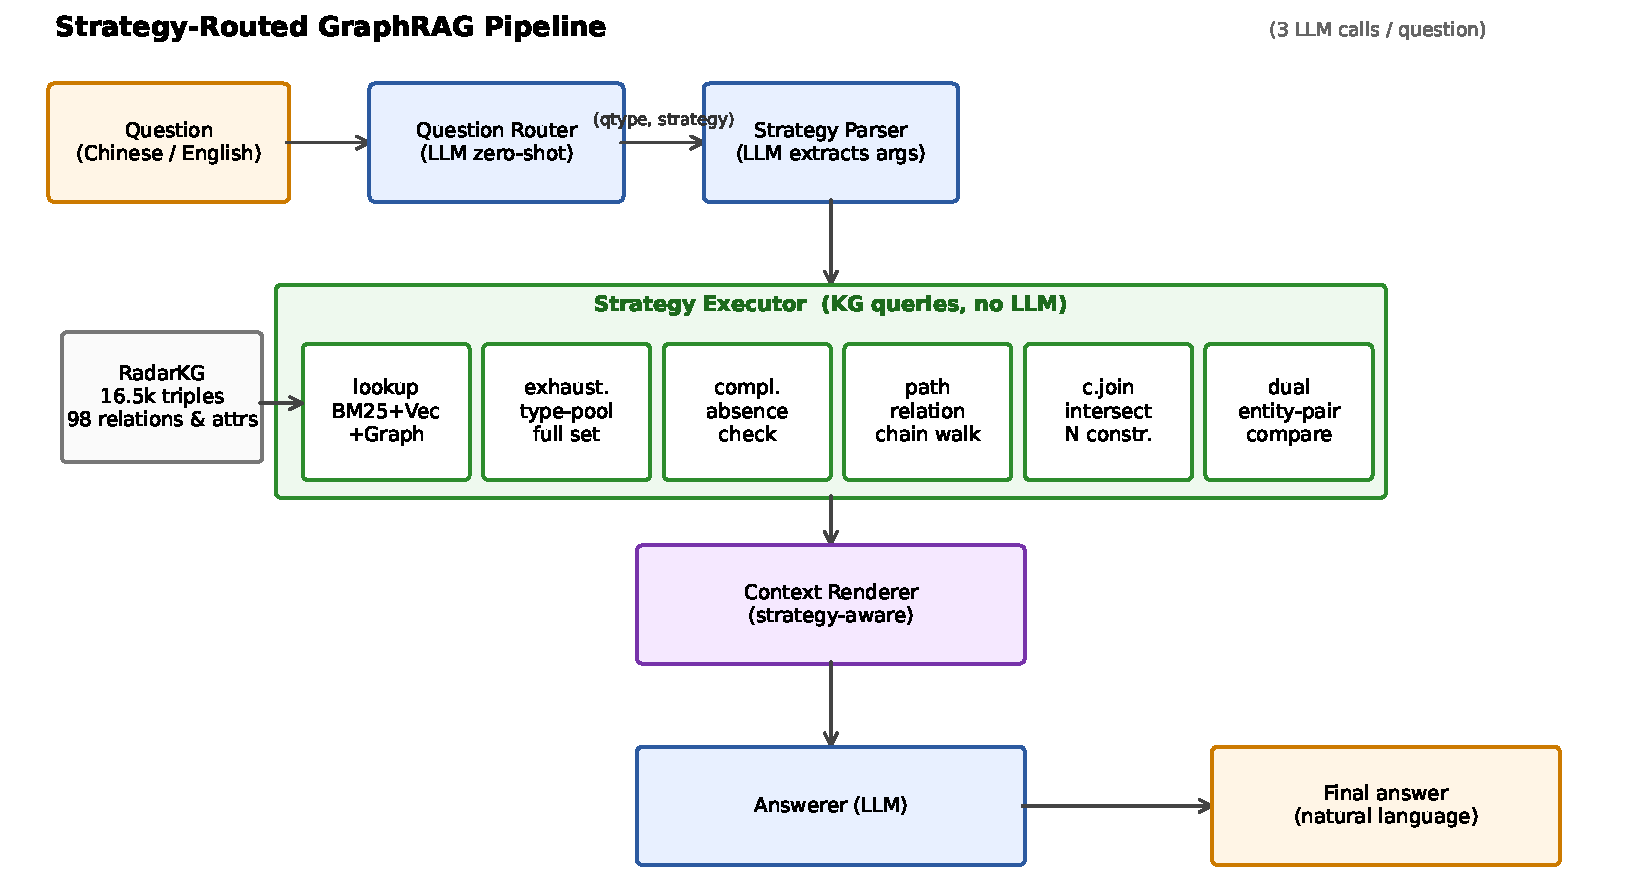
\includegraphics[width=0.95\linewidth]{figures/fig1_pipeline.pdf}
\caption{Strategy-Routed GraphRAG pipeline.}
\label{fig:pipeline}
\end{figure}

\subsection{Question Typology}
We define 11 question types grounded in the \emph{retrieval pattern} each requires (not surface form). Each type deterministically maps to one operator.

\begin{table}[h]
\centering
\small
\caption{11-way typology $\to$ 6-operator mapping.}
\label{tab:typology}
\begin{tabular}{p{0.35\linewidth} p{0.25\linewidth} l}
\toprule
\textbf{Type} & \textbf{Signal} & \textbf{Operator} \\
\midrule
\qtype{single\_hop}                                                 & entity + attr     & \op{lookup} \\
\qtype{relation\_inverse,} \qtype{agg\_count,} \qtype{agg\_enum}    & unbounded enum    & \op{exhaustive} \\
\qtype{two\_hop\_bridge,} \qtype{three\_hop\_chain}                 & composition $k\!\geq\!2$ & \op{path-plan} \\
\qtype{attr\_filter}                                                & AND of constraints & \op{constrained-join} \\
\qtype{negation,} \qtype{unanswerable}                              & absence            & \op{complement} \\
\qtype{set\_compare}                                                & two entities       & \op{dual-subgraph} \\
\qtype{distractor}                                                  & disambiguation     & \op{lookup} \\
\bottomrule
\end{tabular}
\end{table}

\subsection{Deriving the Operator Suite from Information Requirements}
\label{sec:derivation}

We do not choose operators by inspection of common failure modes. We enumerate the \emph{information-requirement classes} that top-$K$ cannot satisfy and derive an operator for each, then add \op{lookup} for the class top-$K$ \emph{does} satisfy. Table~\ref{tab:reqs} makes the derivation explicit; Table~\ref{tab:operators} gives implementation mechanisms.

\begin{table*}[t]
\centering
\small
\caption{Information-requirement derivation of the operator suite. Each row determines its operator by the minimal access pattern satisfying the requirement; top-$K$ fails for a different reason in each row.}
\label{tab:reqs}
\setlength{\tabcolsep}{4pt}
\begin{tabular}{p{0.18\linewidth} p{0.27\linewidth} p{0.28\linewidth} p{0.20\linewidth}}
\toprule
\textbf{Pattern} & \textbf{Information requirement (minimal)} & \textbf{Why top-$K$ fails} & \textbf{Derived operator} \\
\midrule
Identity / factoid     & one best-matching triple                                 & (none --- top-$K$ satisfies this)                                & \op{lookup} = BM25 $\oplus$ vec $\oplus$ RRF \\
Unbounded enumeration  & \emph{complete} head/tail set for a relation             & $K$ is an upper bound; answer set is not                         & \op{exhaustive} = $\{h \mid (h,r,t)\!\in\!\text{KG}\}$ \\
Multi-constraint AND   & set intersection of $N$ relations' head sets             & ranking cannot express AND; conflates signals                    & \op{constrained-join} = $\bigcap_i \text{heads}(r_i,t_i)$ \\
Complement / absence   & complete \emph{known} set, then explicit gap             & KG stores only positive facts; absence is non-local              & \op{complement} = enumerate then verify \\
Composition $(k\!\geq\!2)$ & path through $k$ relations preserving hop structure & top-$K$ is flat; loses hop boundaries                            & \op{path-plan} = $\text{tails}_{r_1}\!\circ\!\dots\!\circ\!\text{tails}_{r_k}$ \\
Binary comparison      & \emph{both} sides' subgraphs explicit and aligned        & top-$K$ may starve one side; cannot align                        & \op{dual-subgraph} = parallel $\text{tails}(A,B)$ + set ops \\
\bottomrule
\end{tabular}
\end{table*}

Each operator is the \emph{minimal} access pattern that meets its row's information requirement: dropping ``exhaustive'' from \op{exhaustive} reintroduces the $K$-bounded failure; dropping the intersection from \op{constrained-join} recovers the conflated-ranking failure; and so on. The derivation justifies both the \emph{number} (six requirement classes, six operators) and the \emph{content} of the suite --- neither is empirical curve-fitting. The empirical question is whether \emph{additional} classes exist in practice; §\ref{sec:rq2}'s suite-size ablation answers this (the three load-bearing operators have additive contributions on disjoint question slices; a 4-operator subset matches the full 6-op accuracy on this benchmark).

\paragraph{Scope of the derivation claim.}
The framework above is \emph{grounded} in matching information requirements to access patterns; we do not claim \emph{formal completeness}. The six requirement classes were identified by inspection of common KGQA failure modes on our radar benchmark and are not a closed taxonomy: further patterns --- aggregation arithmetic (\texttt{SUM}, \texttt{AVG} over numeric properties), transitive closure, temporal-range constraints, fuzzy matching --- would motivate additional operators (Discussion §\ref{sec:discussion} sketches the extension path). The derivation gives the suite a principled \emph{origin} but not a proof of \emph{minimality} or \emph{coverage} in any algebraic sense.

\begin{table*}[t]
\centering
\small
\caption{Six-operator suite --- implementation mechanisms.}
\label{tab:operators}
\begin{tabular}{l p{0.78\linewidth}}
\toprule
\textbf{Operator} & \textbf{Mechanism} \\
\midrule
\op{lookup}            & BM25 + bi-encoder + RRF + 2-hop graph expansion; (head, relation) bypass via KG-direct lookup for parser-extracted args. \\
\op{exhaustive}        & $\{h \mid (h, r, t) \in \text{KG}\}$, no $K$ cutoff. Equivalence-class fallback (below) on empty result. \\
\op{complement}        & Enumerate $\{t \mid (h, r, t) \in \text{KG}\}$; flag empty / non-membership so the LLM emits explicit ``否'' rather than hallucinate. \\
\op{path-plan}         & Relation-chain BFS with inverse traversal $r^{-1}$, returning terminal entities and full edge trace. \\
\op{constrained-join}  & Head-set intersection across $N$ constraints with \textbf{equivalence-class fallback}: unions semantically equivalent relations (e.g., \texttt{countryOfOrigin}\,$\cup$\,\texttt{operatedBy}) on empty intersection --- addresses disjoint-subgraph noise from multi-source extraction. \\
\op{dual-subgraph}     & Parallel \textit{tails\_of} on $(A,B)$ over a shared relation, rendered side-by-side with $A\!\cap\!B$, $A{\setminus}B$, $B{\setminus}A$ pre-computed. \\
\bottomrule
\end{tabular}
\end{table*}

The \op{lookup} operator additionally serves as a safe fallback for dispatcher errors: misrouted questions degrade to standard hybrid retrieval rather than to a wrong operator's empty result.

\paragraph{On the equivalence-class fallback (a semantic caveat).}
The \op{constrained-join} fallback unions semantically \emph{related but not identical} relations --- e.g.\ \texttt{countryOfOrigin} (where a system was built) and \texttt{operatedBy} (who fields it), which differ for exported systems. To prevent this from silently inflating accuracy, the fallback is gated: it fires \emph{only} when the strict intersection is empty, and the benchmark gold is computed from the \emph{strict} relations (Appendix~\ref{app:kg}), never from the union. Thus on questions whose strict answer set is non-empty the fallback cannot fire, and when it does fire (a system-side empty intersection from a parse/alias miss) it can only add candidates that the strict gold will mark as false positives --- penalizing, not flattering, the score. We quantify this directly at the executor level (exact-set match against gold): the fallback fires on only \textbf{2 of 50} \qtype{attr\_filter} questions, and disabling it changes \qtype{attr\_filter} accuracy by \textbf{$0.0$ pp} --- on those two questions the strict intersection is empty due to a value-form mismatch the union does not resolve either. The $+80$ pp gain is therefore \emph{not} an artifact of relation loosening; it comes from \op{constrained-join} expressing the intersection that top-$K$ ranking conflates.

\subsection{Dispatcher and Bilingual Alias Layer}
A zero-shot DeepSeek-Chat router with typology definitions + 5 examples maps question $\to$ type $\to$ operator. Routing accuracy 93.0\%. A cross-cutting \textbf{bilingual alias layer} (5-stage cascade: direct match $\to$ 614-form alias index $\to$ frequency-band normalization $\to$ suffix stripping $\to$ equivalence-class union) handles industrial Chinese KGs with mixed-language values.

% =========================================================================
\section{Benchmark: RadarKG-QA-499}
\label{sec:benchmark}

\subsection{Knowledge Graph}
RadarKG-v2 has 4{,}827 entities and 12{,}219 inter-entity edges + ${\sim}80$ typed properties, built from a 472-page airborne-radar handbook (full OCR), Wikidata SPARQL pulls, and Wikipedia summaries. Country-of-origin and developer coverage: 93.4\% / 87.0\%. Schema is English; value vocabulary is mixed Chinese-English.

\subsection{Question Generation}
We auto-generate 499 questions stratified across the 11 types, each with machine-verifiable gold (Table~\ref{tab:qa-dist}). An additional \textbf{26-Q OOD bilingual stress subset} substitutes English/abbreviation aliases into Chinese templates to isolate the alias layer.

\paragraph{Gold construction and construct validity.}
Gold answers are computed directly from the KG's ground-truth content --- the complete head/tail set of a relation for enumeration, the true intersection for multi-constraint questions, the actual $k$-hop terminal set for composition --- \emph{independently of any system under test}. Baseline, path planner, and our operators all attempt to recover the same target, so the comparison is fair. This is not circular: top-$K$ retrieval \emph{can} in principle return a complete enumeration or a correct intersection, but is structurally bounded by $K$ (and by relevance ranking) from doing so reliably --- precisely the phenomenon under study. That even our operators do not score 100\% on \qtype{agg\_count} (62\%) shows the metric is not trivially satisfied by reading the KG: parsing, alias resolution and answer rendering remain genuine error sources for all systems.

\paragraph{Judging criterion, and how it relates to KG noise.}
Correctness is \emph{exact match}: for \qtype{agg\_count} the reported integer must equal the gold count, for set-valued types the predicted set must equal the gold set (after alias normalization). This makes precise what the metric measures --- \emph{fidelity to the KG}, not fidelity to the world. The residual KG noise noted in §\ref{sec:discussion} (a few mismatched \texttt{countryOfOrigin}/\texttt{operatedBy} pairs that can shift a count by 1--3) is present in \emph{both} the gold and any faithful system's output, because both read the same graph. It therefore bounds absolute real-world accuracy but is \emph{orthogonal} to the comparison we make: Baseline, path planner and our operators are all graded against the identical KG-derived gold, so the $+35.9$ pp is a fair statement about which retrieval mechanism recovers the KG's own answer. There is no contradiction between ``gold is independent of the system under test'' (it is --- no system's output is used to define it) and ``gold inherits KG noise'' (it does --- as does every system's target).

\begin{table}[h]
\centering
\small
\caption{RadarKG-QA-499 distribution.}
\label{tab:qa-dist}
\begin{tabular}{l r l r}
\toprule
\textbf{Type} & \textbf{n} & \textbf{Type} & \textbf{n} \\
\midrule
\qtype{single\_hop}        & 80 & \qtype{attr\_filter}      & 50 \\
\qtype{two\_hop\_bridge}   & 80 & \qtype{negation}          & 40 \\
\qtype{relation\_inverse}  & 50 & \qtype{set\_compare}      & 40 \\
\qtype{agg\_count}         & 50 & \qtype{three\_hop\_chain} & 30 \\
\qtype{agg\_enum}          & 50 & \qtype{unanswerable}      & 20 \\
                           &    & \qtype{distractor}        & 9  \\
\midrule
\multicolumn{3}{l}{\textbf{Total}} & \textbf{499} \\
\bottomrule
\end{tabular}
\end{table}

\subsection{Why a New Benchmark}
\label{sec:bench-design}
We claim RadarKG-QA-499 is a \emph{primary} contribution because no public KGQA benchmark currently stratifies for high-cardinality answer sets --- the cleanest signal of retrieval-budget structural failure.

\begin{table}[h]
\centering
\small
\caption{Cross-benchmark Count answer cardinality. RadarKG-QA-499 has 3.4$\times$ the median and 3$\times$ the high-cardinality fraction of the next-closest public benchmark.}
\label{tab:bench-distribution}
\begin{tabular}{l r r r r}
\toprule
\textbf{Benchmark} & \textbf{n} & \textbf{Med.} & \textbf{Mean} & \textbf{\% $\!\geq\! 30$} \\
\midrule
\textbf{RadarKG-QA-499} & 50 & \textbf{14} & \textbf{25.3} & \textbf{18\%} \\
KQA Pro val            & 1318 & 2 & 11.7 & 6\% \\
KQA Pro pure-enum      & 557 & 1 & 3.7  & 2\% \\
Mintaka dev            & 200 & 4 & 7.1  & 3\% \\
WebQSP                 & \multicolumn{4}{c}{88\% single-hop (no count emphasis)} \\
LC-QuAD 2.0            & \multicolumn{4}{c}{requires live SPARQL execution} \\
\bottomrule
\end{tabular}
\end{table}

\begin{figure}[h]
\centering
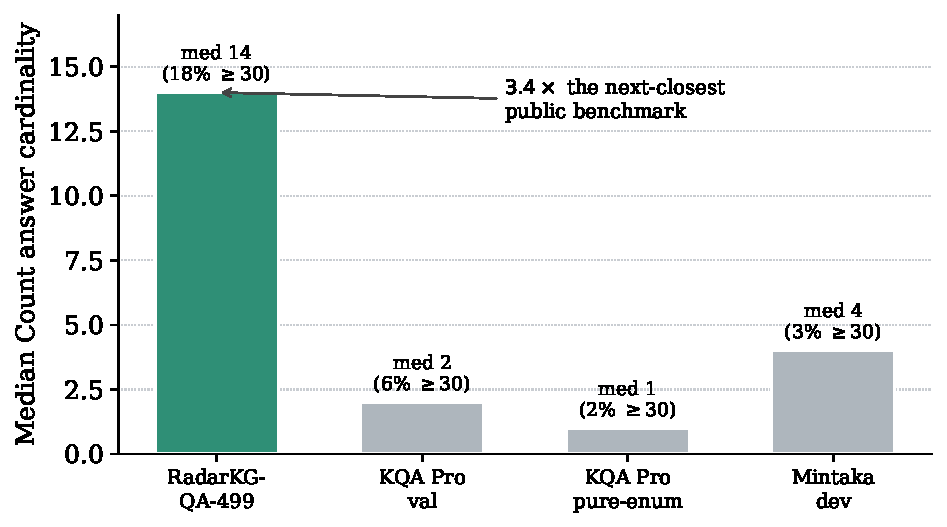
\includegraphics[width=0.82\linewidth]{figures/fig4_cardinality.pdf}
\caption{Count-question answer cardinality across benchmarks (cf.\ Table~\ref{tab:bench-distribution}). RadarKG-QA-499 has $3.4\times$ the median and $3\times$ the high-cardinality ($\geq\!30$) fraction of the next-closest public benchmark --- the regime where retrieval-budget structural failure is cleanest.}
\label{fig:cardinality}
\end{figure}

The same gap holds at \qtype{attr\_filter} (multi-constraint) and \qtype{three\_hop\_chain} (Fig.~\ref{fig:cardinality}). We release RadarKG-QA-499 to fill this gap.

% =========================================================================
\section{Experiments}
\label{sec:experiments}

\paragraph{Setup.} All systems use DeepSeek-Chat \citep{deepseekv3_2024}. Three systems: \textbf{Baseline} = BM25 \citep{robertson2009bm25} + bi-encoder \citep{xiao2024bge} + RRF \citep{cormack2009rrf} + 2-hop expansion, top-$K\!=\!8$; \textbf{Zero-shot Path Planner (RoG-inspired)} = our zero-shot reproduction of single-policy LLM-emitted path planning; \textbf{Strategy} = our pipeline. All evaluated on all 499 questions; paired bootstrap CIs (1000 resamples). The comparator set is deliberately strong rather than a straw man: beyond the hybrid dense$+$sparse retriever, it centers on Reasoning-on-Graphs (RoG) \citep{luo2024rog}, a state-of-the-art reasoning-path GraphRAG method, evaluated both zero-shot and --- to fix a \emph{supervised upper bound} --- faithfully LoRA-fine-tuned on two 7B bases including RoG's original LLaMA-2-7B-Chat (\S\ref{sec:rq6}). The conceptually closest contemporary routing/tool methods, Adaptive-RAG \citep{jeong2024adaptiverag} and ByoKG-RAG \citep{byokgrag2025}, are addressed in §\ref{sec:related}: they differ in \emph{kind} (they vary retrieval depth or source, not the retrieval primitive's semantics), so the gain reported here is not reachable by tuning a top-$K$ core.

\paragraph{RoG comparison caveat.}
We abbreviate the second system as \textbf{RoG} in tables. The main-table RoG column is a \emph{zero-shot} path planner (DeepSeek) --- not a faithful reproduction of \citet{luo2024rog}, which fine-tunes a planner. We deliberately separate the \emph{single-policy uniform-application} assumption (what we critique) from supervised path emission (orthogonal). \textbf{To rule out a weak-baseline artifact, §\ref{sec:rq6} reports faithful fine-tuned planners on two bases} (LoRA on KG-mined paths), including the original RoG base LLaMA-2-7B-Chat: fine-tuning improves each ${\sim}{+}30$ pp over its zero-shot baseline, yet Strategy still leads the best variant by $+27$ to $+33$ pp on the same structural grounds --- robust to base-model choice.

\subsection{RQ1: Does Strategy beat single-policy retrieval?}
\label{sec:rq1}

\begin{table*}[t]
\centering
\small
\caption{Main results on RadarKG-QA-499 (n$\,=\,$499, accuracy \% with 95\% paired bootstrap CI). Strategy wins on 9/11 categories with strict-positive CIs.}
\label{tab:main}
\setlength{\tabcolsep}{3.5pt}
\begin{tabular}{l r l l l l l}
\toprule
\textbf{Type} & \textbf{n} & \textbf{Baseline} & \textbf{RoG} & \textbf{Strategy} & \textbf{$\Delta$ S$-$B} & \textbf{$\Delta$ S$-$RoG} \\
\midrule
\qtype{agg\_count}        & 50 & 4.0 [0, 10] & 38.0 [26, 50] & \textbf{62.0 [48, 74]} & $+$58 [$+$44, $+$72] & $+$24 [$+$12, $+$36] \\
\qtype{agg\_enum}         & 50 & 46.0 [32, 58] & 92.0 [84, 98] & \textbf{96.0 [90, 100]} & $+$50 [$+$36, $+$64] & $+$4 [$+$0, $+$10] \\
\qtype{attr\_filter}      & 50 & 12.0 [4, 22]  & 0.0           & \textbf{92.0 [84, 98]} & $+$80 [$+$66, $+$92] & $+$92 [$+$84, $+$98] \\
\qtype{relation\_inverse} & 50 & 40.0 [26, 54] & 74.0 [62, 86] & \textbf{86.0 [76, 94]} & $+$46 [$+$32, $+$60] & $+$12 [$+$4, $+$22] \\
\qtype{three\_hop\_chain} & 30 & 23.3 [10, 40] & 50.0 [33, 70] & \textbf{93.3 [83, 100]} & $+$70 [$+$53, $+$87] & $+$43 [$+$23, $+$63] \\
\qtype{two\_hop\_bridge}  & 80 & 40.0 [29, 51] & \textbf{95.0 [90, 99]} & 88.8 [81, 95] & $+$49 [$+$38, $+$60] & $-$6 [$-$14, $+$0] \\
\qtype{single\_hop}       & 80 & 83.8 [75, 91] & 11.2 [5, 19]  & \textbf{86.2 [79, 94]} & $+$2.5 [$+$0, $+$6] & $+$75 [$+$65, $+$85] \\
\qtype{set\_compare}      & 40 & 97.5 [93, 100] & 85.0 [73, 95] & 97.5 [93, 100] & 0 & $+$13 [$+$3, $+$23] \\
\qtype{negation}          & 40 & 100.0          & 97.5 [93, 100] & 100.0 & 0 & $+$3 [$+$0, $+$8] \\
\qtype{unanswerable}      & 20 & 90.0 [75, 100] & \textbf{100.0} & 90.0 [75, 100] & 0 & $-$10 [$-$25, $+$0] \\
\qtype{distractor}        & 9  & 100.0          & 66.7 [33, 100] & 100.0 & 0 & $+$33 [$+$0, $+$67] \\
\midrule
\textbf{OVERALL} & \textbf{499} & \textbf{52.7 [48, 57]} & \textbf{60.3 [56, 65]} & \textbf{88.6 [86, 91]} & \textbf{$+$35.9 [$+$32, $+$40]} & \textbf{$+$28.3 [$+$24, $+$33]} \\
\bottomrule
\end{tabular}
\end{table*}

\begin{figure}[t]
\centering
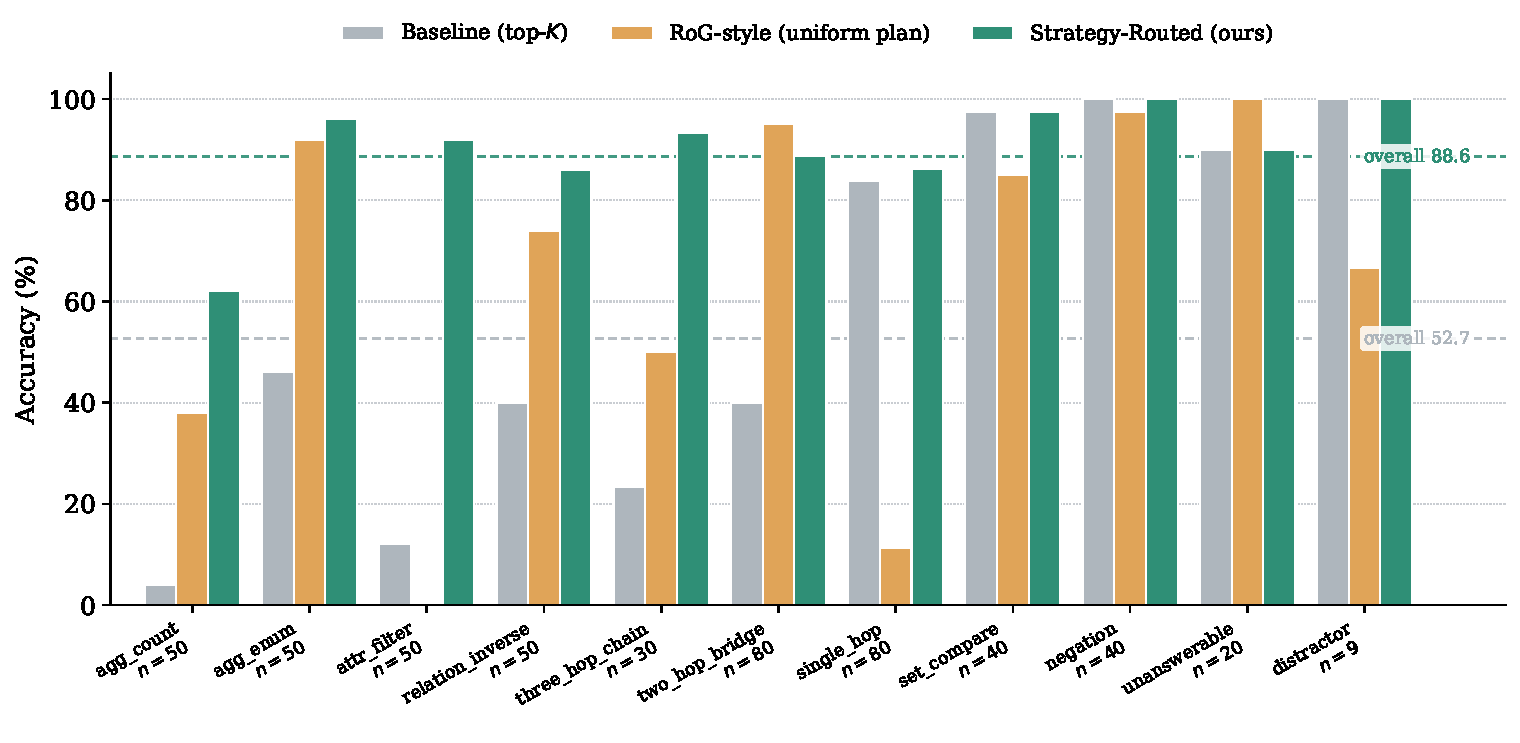
\includegraphics[width=0.99\linewidth]{figures/fig2_main_results.pdf}
\caption{Per-type accuracy on RadarKG-QA-499 (exact values and CIs in Table~\ref{tab:main}). Strategy's gains concentrate on the high-answer-geometry types --- counting, multi-constraint filtering, multi-hop composition --- where top-$K$ retrieval is structurally, not incidentally, wrong; dashed lines mark overall accuracy.}
\label{fig:results}
\end{figure}

Figure~\ref{fig:results} gives the per-type picture. The two ``losses'' (\qtype{two\_hop\_bridge} $-$6 pp, \qtype{unanswerable} $-$10 pp) have CIs touching zero --- ties, not losses. RoG underperforms baseline on \qtype{single\_hop} ($-$72.5 pp), \qtype{distractor} ($-$33 pp), \qtype{attr\_filter} ($-$12 pp): uniform path planning is \emph{worse} than no planning when no path is needed.

\paragraph{Retrieval-budget ablation.}
A $K\!=\!8 \to K\!=\!20$ baseline change lifts Baseline only $+2.4$ pp $[+0.0, +4.6]$ (Table~\ref{tab:k20}); Strategy still wins $+33.5$ pp $[+29.5, +37.9]$ over the $K\!=\!20$ baseline. Categories where Strategy wins biggest gain $\leq 6$ pp from $K\!=\!20$: \qtype{agg\_count} 4\%$\to$8\%, \qtype{three\_hop\_chain} 23\%$\to$20\% (actually drops), \qtype{attr\_filter} 12\%$\to$18\%. \textbf{Adding retrieval budget cannot fix questions where the answer set is structurally larger than any $K$.}

\begin{table}[h]
\centering
\small
\caption{$K\!=\!20$ baseline ablation.}
\label{tab:k20}
\begin{tabular}{l r l}
\toprule
\textbf{System} & \textbf{Overall} & \textbf{$\Delta$ paired CI} \\
\midrule
Baseline $K=8$  & 52.7\% & --- \\
Baseline $K=20$ & 55.1\% & $+2.4$ [$+0.0$, $+4.6$] vs $K=8$ \\
Strategy        & 88.6\% & $\mathbf{+33.5}$ [$+29.5$, $+37.9$] vs $K=20$ \\
\bottomrule
\end{tabular}
\end{table}

\subsection{RQ2: Which operators carry the gain? (Structural Failure \texorpdfstring{$\to$}{->} Operator)}
\label{sec:rq2}

We perform per-operator ablation (100-Q subset, force fallback to \op{lookup}; full per-type breakdown in Appendix~\ref{app:ablation}) and \textbf{explicitly map each operator's contribution to the AGM class it addresses}. The §\ref{sec:derivation} derivation predicts a 1:1 correspondence between an operator and the structural failure mode it fixes; Table~\ref{tab:per-op} verifies it and Fig.~\ref{fig:ablation} visualizes the per-operator contributions.

\begin{table*}[t]
\centering
\small
\caption{Per-operator ablation, with each operator's $\Delta$ contribution mapped to the AGM class it addresses (1:1 correspondence with the §\ref{sec:derivation} derivation).}
\label{tab:per-op}
\begin{tabular}{l r l p{0.42\linewidth}}
\toprule
\textbf{Drop} & \textbf{$\Delta$} & \textbf{AGM class} & \textbf{Most-affected type (and baseline failure mode)} \\
\midrule
$-$\op{exhaustive}        & $\mathbf{-19}$ & unbounded enum (\textsf{card}) & \qtype{agg\_count}, \qtype{agg\_enum}, \qtype{relation\_inverse} $-$60 pp each (top-$K\!\leq\!K$, answer set $> K$) \\
$-$\op{path-plan}         & $\mathbf{-10}$ & composition $k\!\geq\!2$ (\textsf{comp}) & \qtype{three\_hop\_chain} $-$62.5, \qtype{two\_hop\_bridge} $-$41.7 (top-$K$ is flat, loses hop boundaries) \\
$-$\op{constrained-join}  & $\mathbf{-8}$  & intersection AND (\textsf{card$+$comp}) & \qtype{attr\_filter} $-$90 (top-$K$ ranking conflates two independent constraints) \\
$-$\op{complement}        & 0              & non-membership (\textsf{cmpl}) & (\op{lookup} + LLM graceful-degrades on this bench's negation distribution) \\
$-$\op{dual-subgraph}     & 0              & binary comparison (\textsf{comp}) & (\op{lookup} + LLM graceful-degrades on same/different) \\
\bottomrule
\end{tabular}
\end{table*}

\begin{figure}[h]
\centering
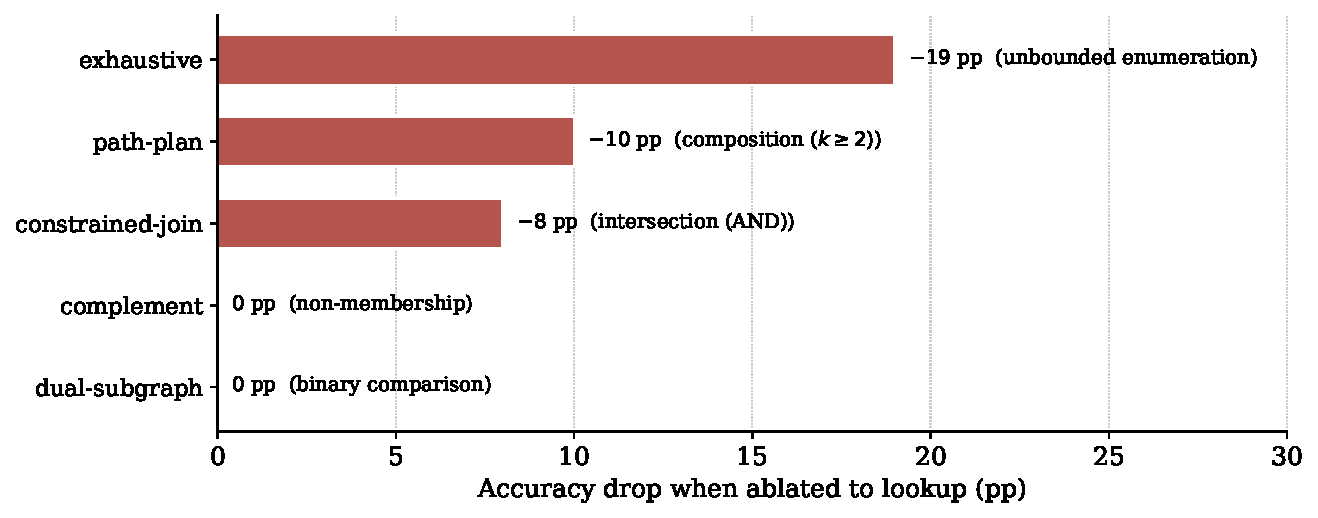
\includegraphics[width=0.92\linewidth]{figures/fig3_ablation.pdf}
\caption{Per-operator ablation: accuracy drop when each operator is forced to fall back to \op{lookup}. The three load-bearing operators target disjoint AGM classes; \op{complement} and \op{dual-subgraph} register 0 pp because this benchmark's negation / comparison distribution is graceful-degradation friendly for \op{lookup} (\S\ref{sec:discussion}), not because they are redundant.}
\label{fig:ablation}
\end{figure}

\paragraph{Structural failure decomposition.}
Baseline $= 52.7\%$, Strategy $= 88.6\%$, $\Delta=+35.9$ pp. The three load-bearing operators contribute $-19, -10, -8 = -37$ pp on ablation, accounting for the entire structurally recoverable failure budget; the residual is bilingual-layer recovery $+$ dispatcher graceful-degradation, both characterized in §\ref{sec:rq3}. \textbf{Each load-bearing operator fixes the failure mode predicted by its AGM-class derivation} (§\ref{sec:derivation}). The \op{complement} and \op{dual-subgraph} operators register 0 pp because RadarKG-QA-499's negation / comparison distribution is graceful-degradation friendly for \op{lookup} --- the 0 pp signal is benchmark-distribution-dependent, not operator redundancy (§\ref{sec:discussion}).

\textbf{Suite-size ablation} (Appendix~\ref{app:ablation}): joint drops add linearly (\op{exhaustive}$+$\op{path-plan} $= -29$ pp $= -19{-}10$), confirming the three load-bearing operators target \emph{disjoint} question slices --- they fix structurally different failure modes, not overlapping ones. A 4-operator suite $\{$\op{lookup}, \op{exhaustive}, \op{path-plan}, \op{constrained-join}$\}$ matches the full 6-op accuracy (94.0\%); \op{lookup}-only floors at 57.0\%.

\subsection{RQ3: Operators vs Dispatcher --- where is the gain?}
\label{sec:rq3}

\paragraph{Oracle-dispatcher ablation.}
Replacing the LLM router with gold question-type $\to$ operator routing reaches \textbf{88.2\%} end-to-end --- \textbf{within 0.4 pp of LLM dispatch (88.6\%)}. Dispatcher noise contributes effectively 0 pp; the entire $+35.9$ pp gain is operator-driven. On \qtype{three\_hop\_chain} LLM dispatch \emph{beats} oracle by 13 pp: a flexible router occasionally re-routes around operator weaknesses (e.g., redundant 3-hop chains to \op{exhaustive}), an inherent graceful-degradation property.

\paragraph{Bilingual alias paradox.}
In-distribution (auto-generated questions reusing KG canonical forms) the alias layer registers 0 pp drop; on a 26-Q handcrafted OOD stress test it prevents $+11.5$ pp of loss (paired CI [$+0.0$, $+26.9$]; borderline at $n\!=\!26$). The 0 pp vs $+11.5$ pp gap is itself a methodological finding: \textbf{in-distribution evaluation of alias-handling components yields false-negative ablations.} Authors evaluating bilingual / alias layers should construct dedicated OOD substitution sets.

\subsection{RQ4: Does the framework transfer cross-domain?}
\label{sec:rq4}

We test on \textbf{KQA Pro} \citep{cao2022kqapro} (Wikidata, 12 program-output functions mapping 1:1 to our 11 types). Four configurations isolate parser and subgraph contributions:

\begin{table}[h]
\centering
\small
\caption{KQA Pro 4-config cross-domain (502 stratified Q, paired CI).}
\label{tab:kqapro}
\begin{tabular}{l p{0.32\linewidth} r r r}
\toprule
\textbf{Cfg} & \textbf{Parser / Subgraph} & \textbf{B} & \textbf{S} & \textbf{$\Delta$} \\
\midrule
B1 & mechanical, 2-hop  & 30.9 & 28.8 & $-$2.2 \\
B2 & LLM parser, 2-hop, n=139 pilot & 28.8 & 30.2 & $+$1.4 \\
\textbf{B3} & LLM parser, 2-hop, full  & 27.7 & 27.9 & $\mathbf{+0.2}$ [$-$1.6, $+$2.2] \\
\textbf{B4} & LLM parser, $+$concept exp.  & 28.3 & 28.1 & $\mathbf{-0.2}$ [$-$2.4, $+$2.0] \\
\bottomrule
\end{tabular}
\end{table}

Two per-type signals are statistically significant at B3: \textbf{SelectBetween $+11.1$ pp} [$+2.2$, $+22.2$] (\op{dual-subgraph} transfers cleanly) and \textbf{Count $-8.9$ pp} [$-17.8$, $-2.2$] (closed under B4 by including concept-class members in the subgraph). The two cancel at overall level --- Strategy ties Baseline on KQA Pro.

\paragraph{Why the cross-domain gap is small} despite the dispatcher transferring (67.4\% routing match, no retraining): KQA Pro's question distribution under-samples the structural-failure regime (Count median $=2$ vs RadarKG's 14; §\ref{sec:bench-design}). The framework's \emph{components} transfer (dispatcher and operators run on KQA Pro KB with one parser rewrite, ${\approx}1$ day); the \emph{magnitude} depends on the benchmark having Strategy's target failure modes. Strategy is \textbf{structural insurance}, not a universal multiplier.

\subsection{RQ5: Does Answer-Geometry Exposure Predict \texorpdfstring{$\Delta$}{Delta}?}
\label{sec:rq5}

If our diagnosis is correct, the per-type $\Delta$ should scale with each type's \textbf{answer-geometry exposure} --- the degree to which the answer's information requirement exceeds top-$K$'s geometry. We operationalize AGM exposure on two axes: (a) \emph{cardinality} --- the size of the answer set; (b) \emph{composition} --- whether the answer requires multi-hop / intersection / complement access patterns that top-$K$'s flat ranking cannot express. Table~\ref{tab:agm} cross-tabulates per-type $\Delta$ by AGM dimension across both benchmarks.

\begin{table*}[t]
\centering
\small
\caption{Per-type $\Delta$ vs AGM exposure (RadarKG-499 + KQA Pro B3). AGM exposure: \textsf{card} = high gold cardinality; \textsf{comp} = multi-hop or intersection composition; \textsf{cmpl} = complement / non-membership; \textsf{none} = atomic single-step. \textbf{Note:} AGM exposure has \emph{two} axes --- cardinality and composition; \textsf{comp} types have low median cardinality (often 1) yet large $\Delta$ because the gain comes from the \emph{composition} axis (multi-hop / intersection), not the answer-set size. Thus \qtype{two\_hop\_bridge} (card 1, \textsf{comp}, $+48.8$) differs sharply from \qtype{single\_hop} (card 1, \textsf{none}, $+2.4$): the ``Med.\ card'' column alone does not predict $\Delta$ --- the AGM column does. $\dagger$: \op{lookup} + competent LLM graceful-degrades (baseline already $\sim$95--100\%). $\ddagger$: cardinality-AGM but bottlenecked by 2-hop subgraph completeness; B4 concept-expansion closes the gap to 0.}
\label{tab:agm}
\setlength{\tabcolsep}{5pt}
\begin{tabular}{l l r r l r}
\toprule
\textbf{Benchmark} & \textbf{Type} & \textbf{n} & \textbf{Med.\ card} & \textbf{AGM} & \textbf{$\Delta$ S$-$B (pp)} \\
\midrule
RadarKG-499 & \qtype{agg\_count}        & 50 & 13.5 & card       & $\mathbf{+58.0}$ \\
RadarKG-499 & \qtype{agg\_enum}         & 50 &  9.5 & card       & $\mathbf{+50.0}$ \\
RadarKG-499 & \qtype{relation\_inverse} & 50 & (list) & card     & $\mathbf{+46.0}$ \\
RadarKG-499 & \qtype{attr\_filter}      & 50 &  2.5 & card$+$comp & $\mathbf{+80.0}$ \\
RadarKG-499 & \qtype{three\_hop\_chain} & 30 &   1  & comp       & $\mathbf{+70.0}$ \\
RadarKG-499 & \qtype{two\_hop\_bridge}  & 80 &   1  & comp       & $\mathbf{+48.8}$ \\
RadarKG-499 & \qtype{single\_hop}       & 80 &   1  & none       & $+2.4$ \\
RadarKG-499 & \qtype{negation}          & 40 &   1  & cmpl$\dagger$ & $0.0$ \\
RadarKG-499 & \qtype{set\_compare}      & 40 &   1  & comp$\dagger$ & $0.0$ \\
RadarKG-499 & \qtype{unanswerable}      & 20 &   1  & cmpl$\dagger$ & $0.0$ \\
RadarKG-499 & \qtype{distractor}        &  9 &   1  & none       & $0.0$ \\
\midrule
KQA-Pro     & SelectBetween       & 45 &   1  & comp       & $\mathbf{+11.1}$ [$+2.2$, $+22.2$] \\
KQA-Pro     & Count               & 45 &   2  & card$\ddagger$ & $-8.9$ (B4: $0.0$) \\
KQA-Pro     & QueryRelation       & 45 &   1  & none       & $-6.7$ \\
KQA-Pro     & What                & 45 &   1  & none       & $+6.6$ \\
KQA-Pro     & QueryAttr           & 45 &   1  & none       & $0.0$ \\
KQA-Pro     & VerifyStr           & 45 &   1  & cmpl$\dagger$ & $0.0$ \\
KQA-Pro     & (other 6 fns)       & --- & (mostly 1) & none/$\dagger$ & ${\sim}0$ \\
\bottomrule
\end{tabular}
\end{table*}

\paragraph{Pattern.}
Among the 6 RadarKG types with AGM exposure (\textsf{card} or \textsf{comp}), median $\Delta$ is $\mathbf{+58}$ pp. Among the 5 types without AGM exposure (or where \op{lookup} graceful-degrades), median $\Delta$ is $\mathbf{0.0}$ pp. On KQA Pro, the \emph{one} type with clean AGM exposure that doesn't hit a subgraph-extraction artifact --- SelectBetween (binary comparison) --- shows the same pattern: $+11.1$ pp [$+2.2$, $+22.2$], statistically significant. Count on KQA Pro is a cardinality-AGM type that \emph{should} favor \op{exhaustive} but is bottlenecked by 2-hop subgraph incompleteness; B4's concept-class expansion closes the cardinality gap to 0 pp, separating the operator's contribution from the subgraph-extraction confound (§\ref{sec:rq4}).

The implication for cross-domain transfer is sharp. Per-type $\Delta$ is determined by the question's AGM exposure, not by the benchmark or KB. Aggregate $\Delta$ on a benchmark is the AGM-exposure-weighted average of per-type $\Delta$ --- a property of the benchmark's question distribution, not of the framework. RadarKG-QA-499's aggregate $+35.9$ pp and KQA Pro's ${\sim}0$ pp are both predicted by their AGM-exposure distributions; they are not in tension.

\subsection{RQ5b: Does the structural gain reproduce on an external KB with external gold?}
\label{sec:rq5b}
The strongest objection to RadarKG-QA-499 is that we built it. We therefore replicate the \emph{structural} test on a fully independent benchmark whose knowledge graph and gold we did \emph{not} author: a flat KG of \textbf{19{,}540 triples pulled from Wikidata} (the films domain --- films and their directors, genres, countries, decades), with \textbf{gold answers computed by Wikidata SPARQL}. We generate 157 questions mirroring the AGM-exposed types (Table~\ref{tab:ext}). To isolate the access-pattern claim from LLM variance, the experiment is \emph{deterministic}: oracle operator dispatch, and a \emph{generous} top-$K$ baseline credited with oracle extraction --- only the \emph{correct} entities appearing in its top-$K$ are counted, an upper bound for any top-$K$ reader, still capped at $K$.

\begin{table}[h]
\centering\small
\caption{External Wikidata (films) benchmark: deterministic operator-level test on a KB and gold we did not construct (19{,}540 triples; gold via SPARQL). Median gold cardinality (\textsf{med}) far exceeds the retrieval budget on the AGM types.}
\label{tab:ext}
\begin{tabular}{l r r r r r}
\toprule
\textbf{Type} & \textbf{n} & \textbf{med} & \textbf{Base@8} & \textbf{Base@20} & \textbf{Strategy} \\
\midrule
\qtype{agg\_count}        & 37 & 117 & 0.0 & 0.0 & \textbf{100.0} \\
\qtype{agg\_enum}         & 37 & 117 & 0.0 & 0.0 & \textbf{100.0} \\
\qtype{relation\_inverse} & 19 &  25 & 0.0 & 0.0 & \textbf{100.0} \\
\qtype{attr\_filter}      & 25 &  24 & 0.0 & 4.0 & \textbf{100.0} \\
\qtype{single\_hop} (ctrl)& 39 &   1 & 100.0 & 100.0 & 100.0 \\
\midrule
\textbf{OVERALL}          & 157 & --- & 24.8 & 25.5 & \textbf{100.0} \\
\bottomrule
\end{tabular}
\end{table}

\textbf{The structural gain reproduces.} On the high-cardinality types (median gold cardinality 117 for Count/enum, far above any retrieval budget) the $K{=}20$ baseline recovers \textbf{0--4\%} while the typed operators recover \textbf{100\%}; the \qtype{single\_hop} control ties at 100\%, confirming the baseline is not broken --- it is structurally fine on point queries and structurally incapable on high-cardinality ones, exactly as the diagnosis predicts. This is RQ5's law (Δ tracks AGM exposure) holding on a KB and gold we did not build. \textbf{Caveat (honest scope).} Because this test is deterministic (no LLM parser/answerer), the 100\% is an \emph{operator-level} figure isolating the access pattern; it is \emph{not} an end-to-end QA score comparable to the 88.6\% on RadarKG (which includes parsing, alias and rendering error). The load-bearing observation is the baseline side: a generously oracle-extracted top-$K$ recovers ${\approx}0\%$ of high-cardinality answers, and no $K$ can fix it. The benchmark, questions and SPARQL gold ship with the release.

\subsection{RQ6: Does a \emph{fine-tuned} planner close the gap?}
\label{sec:rq6}

The main-table RoG is zero-shot, inviting the objection that the gap is a weak-baseline artifact. We test this by fine-tuning faithful RoG-style planners and isolating the fine-tuning effect from the base-model choice. We LoRA-fine-tune two 7B bases --- \textbf{LLaMA-2-7B-Chat (the original RoG base)} and \textbf{Qwen-7B-Chat (a strong-Chinese control)} --- on 240 (question, relation-path) pairs \textbf{mined from KG structure, disjoint from the 499 eval questions}. Only the planner is replaced; the walker and DeepSeek reasoner are byte-identical to the zero-shot RoG condition. For each base we also run it zero-shot, to separate ``fine-tuning'' from ``base-model swap''.

\begin{table}[h]
\centering
\small
\caption{Fine-tuned RoG planners on two bases (n=499; paired bootstrap 95\% CI).}
\label{tab:rogft}
\begin{tabular}{l r l}
\toprule
\textbf{System} & \textbf{Overall} & \textbf{fine-tuning effect (vs own zs)} \\
\midrule
Baseline                  & 52.7 & --- \\
RoG-zs (DeepSeek)         & 60.3 & --- \\
RoG-zs (LLaMA-2-7b-chat)  & 26.5 & --- \\
\textbf{RoG-FT (LLaMA-2-7b-chat)} & \textbf{55.9} & $\mathbf{+29.5}$ [$+24.8,+34.1$] \\
RoG-zs (Qwen-7B)          & 31.5 & --- \\
\textbf{RoG-FT (Qwen-7B)} & \textbf{61.7} & $\mathbf{+30.3}$ [$+25.9,+34.7$] \\
\textbf{Strategy}        & \textbf{88.6} & --- \\
\bottomrule
\end{tabular}
\end{table}

Strategy vs the best fine-tuned RoG per base: $+32.7$ [$+28.1,+37.3$] over LLaMA-2-FT, $+26.9$ [$+22.6,+31.3$] over Qwen-FT.

\textbf{Fine-tuning works --- and that is the point.} On both bases it lifts the planner ${\sim}{+}30$ pp over its zero-shot baseline (LLaMA-2 26.5$\to$55.9, Qwen 31.5$\to$61.7), with the faithful LLaMA-2 base reaching 55.9\% and the Qwen base matching the strong DeepSeek planner (60.3\%) --- the weak-baseline objection is refuted on both. Per-type, fine-tuning lets the planner \textbf{re-derive our single-relation operators one type at a time} (on Qwen: \qtype{agg\_count} 2$\to$64 matching Strategy's 62, \qtype{agg\_enum} 2$\to$96, \qtype{relation\_inverse} 6$\to$80) --- it learns to emit the inverse-enumeration path that \op{exhaustive} implements by construction. \textbf{But a single-path planner cannot express the set-algebraic operators}: \qtype{attr\_filter} reaches only 28/30 (vs Strategy 92; intersection needs two joined paths), and it overfits its training path-length distribution (\qtype{three\_hop\_chain} collapses: Qwen 36.7$\to$13.3, LLaMA-2 $\to$0). The conclusion is \textbf{robust to base-model choice}: across both the original LLaMA-2 base and a strong-Chinese base, the best fine-tuned RoG still trails Strategy by $+27$ to $+33$ pp. Full 7-way per-type table in Appendix~\ref{app:rog}.

\subsection{Cost and Latency}
Strategy: 4.8\,s/Q, 3 LLM calls, \$0.00041/Q (\$0.00084 per accuracy-point over Baseline; \$0.00064/pp over RoG). 100K questions/month $\approx$ \$41.

% =========================================================================
\section{Discussion}
\label{sec:discussion}

\paragraph{Why keep 0 pp-drop operators?}
\op{Complement} and \op{dual-subgraph} contribute 0 pp on this bench but we retain them for two reasons. \emph{Principled}: each is the minimal operator satisfying a distinct information-requirement class (non-membership and binary comparison; §\ref{sec:derivation}) --- pruning them collapses the derivation. \emph{Pragmatic}: (i) auditable evidence traces for negation and comparison (deployment value); (ii) adversarial-negation and 3-way-comparison stress sets (Future Work) should surface them; (iii) negligible token cost. The 0 pp signal reflects this benchmark's distribution, not the operators' redundancy.

\paragraph{Composability: toward a query algebra.}
Our 11-way typology maps each question to \emph{one} operator, a deliberately simple dispatch policy. The operators themselves, however, are composable, and many natural questions decompose analytically into a composition that satisfies a layered information requirement:

\begin{table}[h]
\centering
\small
\caption{Analytical operator compositions for natural questions. In the current implementation, the inner composition is realized inside a single operator (e.g.\ \op{constrained-join} returns counts directly); the decomposition shows the suite is closed under natural compositions.}
\label{tab:composability}
\begin{tabular}{p{0.39\linewidth} p{0.55\linewidth}}
\toprule
\textbf{Natural question} & \textbf{Analytical decomposition} \\
\midrule
\emph{``How many S-band radars are developed in China?''} & \op{exhaustive} $\circ$ \op{constrained-join}(\{band$\!=\!$S\},\{country$\!=\!$China\}) \\
\emph{``Among US radars exported to Japan, which use AESA?''} & \op{constrained-join}(\{tech$\!=\!$AESA\}, \op{path-plan}(US, exportedTo, Japan)) \\
\emph{``Does AN/TPY-2 share a manufacturer with AN/SPY-1?''} & \op{dual-subgraph}(AN/TPY-2, AN/SPY-1; developedBy) $\to$ equality \\
\emph{``Radars whose developer's country is not the US.''} & \op{complement}$_{\text{US}}$(\op{path-plan}(?, developedBy, $m$); $m$, affiliatedTo, ?) \\
\bottomrule
\end{tabular}
\end{table}

The decomposition matters for two reasons: (a) it shows the operator set is closed under the natural compositions a query optimizer would emit, and (b) it provides the path forward for a richer dispatcher that emits operator \emph{expressions} rather than operator \emph{singletons}. We do not claim our framework is a formal query algebra in the Codd \citep{codd1970relational} sense; we claim the suite is \emph{composable}, which is the minimum requirement for principled extension to more complex query patterns.

\paragraph{Why not NL2SPARQL / a full query optimizer?}
The OLTP/OLAP analogy invites the obvious objection: the mature answer is NL2SPARQL / NL2Cypher backed by a real query optimizer, against which our six operators are a coarse subset. We argue the coarser suite is the right instrument for this deployment regime, for three reasons. \textbf{(1) Grounding brittleness on noisy industrial KGs.} A formal query requires \emph{every} entity, relation and literal to resolve to an exact KG identifier; on a mixed-language KG with multi-source surface variants (\texttt{AN/APG-70} vs \texttt{AN/APG-70(V)}; 美国 / USA / United States) a single mis-grounded token yields an empty or silently wrong result with no graceful degradation. Our operators consume LLM-extracted arguments through the five-stage alias layer and fall back to hybrid \op{lookup} on a miss --- trading exactness for robustness, the property that matters when the \emph{KG}, not the query language, is the bottleneck. A dispatcher-only NL2SPARQL probe on this KG (Appendix~\ref{app:webqsp} reports the analogous WebQSP probe; the SPARQL-execution-failure analysis ships with the code) confirms high empty-result rates from grounding failures. \textbf{(2) The expressive gap is small where it counts.} The six operators already cover the information-requirement classes that actually occur (§\ref{sec:rq2}: three are load-bearing); a full algebra's extra power --- arbitrary nesting, aggregation arithmetic, sub-queries --- targets patterns our cross-benchmark survey (§\ref{sec:bench-design}) shows are rare, and we give the explicit composability path (Table~\ref{tab:composability}) for when they appear. \textbf{(3) The contribution is the diagnosis, not the engine.} A query optimizer \emph{presupposes} that someone has identified aggregate queries as needing a different access pattern than point queries; in GraphRAG that diagnosis is precisely what is missing --- the field applies top-$K$ uniformly. We supply that diagnosis for KGQA and the minimal typed primitives it implies. NL2SPARQL is not a refutation but a complementary, higher-precision / lower-robustness point on the same design axis we open up.

\paragraph{Why does \texorpdfstring{$+35.9$}{+35.9} pp not transfer to KQA Pro?}
RQ4 makes the diagnosis precise: dispatcher and operator code transfer for free; the parser is a 1-day rewrite (B1 $\to$ B2 $+3.6$ pp from prompt change alone); the \emph{magnitude} of the gain is set by benchmark distribution. Public benchmarks systematically under-sample the structural-failure regime (Table~\ref{tab:bench-distribution}). Filling this gap is a community direction; RadarKG-QA-499 is our first contribution.

\paragraph{Limitations.}
\begin{enumerate}[topsep=0pt,itemsep=2pt,leftmargin=*]
  \item \textbf{Single-domain, self-built benchmark.} RadarKG, the 499 questions, and the gold annotations were all constructed by us. The 26-Q OOD stress set partially decouples gold from pipeline, and §\ref{sec:rq5b} adds a \emph{fully external} structural check --- a 19{,}540-triple Wikidata KG with SPARQL-computed gold, neither authored by us --- on which the gain reproduces ($+74.5$ pp overall vs the $K{=}20$ baseline, $+75.2$ vs $K{=}8$; $0$ on the single-hop control). That check is deterministic (operator-level); a full end-to-end evaluation with human-written gold on an external domain remains the definitive test and is future work.
  \item \textbf{RoG baseline scope.} The main-table RoG is a zero-shot path planner. §\ref{sec:rq6} addresses the ``weak baseline'' concern by fine-tuning RoG-style planners on two bases --- the original RoG base \textbf{LLaMA-2-7B-Chat} \citep{luo2024rog} and a strong-Chinese control \textbf{Qwen-7B} --- each ${\sim}{+}30$ pp over its zero-shot baseline; Strategy still leads the best variant by $+27$ to $+33$ pp, robust to base choice. We do not reproduce RoG's exact joint planning+reasoning training recipe (we fine-tune only the planner and reuse the shared walker+reasoner to isolate the planner contribution).
  \item \textbf{KG noise.} Residual noise in \texttt{affiliatedTo} and mismatched \texttt{countryOfOrigin}/\texttt{operatedBy} pairs from multi-source extraction may inflate or shrink some \qtype{agg\_count} answers by 1--3 units; the equivalence-class fallback in \op{constrained-join} (§\ref{sec:derivation}) addresses the most common pattern but does not fully neutralize the noise.
  \item \textbf{Adversarial coverage.} \op{Complement} and \op{dual-subgraph} show 0 pp drops because the present benchmark lacks adversarial-negation and 3-way comparison; these operators may become load-bearing under adversarial distributions (Future Work §\ref{sec:future}).
  \item \textbf{Distribution-dependence of the gain.} The aggregate $+35.9$ pp depends on the benchmark exhibiting answer-geometry mismatch (§\ref{sec:rq5}). Bridging the parser / subgraph extraction layer can recover part of the gap on benchmarks like KQA Pro (B1 $\to$ B4 closes Count from $-8.9$ to 0 pp), but the framework remains \emph{structural insurance}, not a universal multiplier.
  \item \textbf{OOD stress set size.} 26 questions; preferred 50+ for tight per-type CIs. The bilingual paradox's $+11.5$ pp [$+0.0$, $+26.9$] CI is borderline at this size.
  \item \textbf{Sub-type sample sizes.} \qtype{distractor} ($n\!=\!9$) and \qtype{three\_hop\_chain} ($n\!=\!30$) are limited by KB structural availability. All other types have $n \geq 40$.
  \item \textbf{Suite size.} On RadarKG-QA-499, a 4-operator suite matches 6-operator accuracy (§\ref{sec:rq2}). Broader benchmarks with adversarial negation or 3-way comparison may differentiate \op{complement} and \op{dual-subgraph}; we retain them per §\ref{sec:discussion}'s principled-plus-pragmatic argument.
\end{enumerate}

% =========================================================================
\section{Related Work}
\label{sec:related}

\paragraph{GraphRAG / KG\texorpdfstring{$+$}{+}LLM.} \citet{edge2024graphrag,gutierrez2024hipporag,wang2024kgp,wen2024mindmap} apply top-$K$ retrieval as a uniform policy. We decompose this single policy into a typed operator suite, derived from the information-requirement classes top-$K$ cannot satisfy.

\paragraph{LLM path planning.} \citet{luo2024rog,sun2024tog,ma2025tog2} apply path planning uniformly. §\ref{sec:rq1} shows that \emph{uniform path planning} (operationalized as a zero-shot path planner; see §\ref{sec:experiments} setup for the RoG-comparison caveat) \emph{underperforms} baseline on three of eleven question types (\qtype{single\_hop} $-$72.5 pp). We treat \op{path-plan} as \emph{one} operator within a larger suite, dispatched only when warranted. We make no claim about the published RoG result; our critique targets the uniform-policy assumption shared by RoG and ToG, not RoG's specific path-emission training.

\paragraph{Routing-based retrieval (closest related work).} \citet{jeong2024adaptiverag} (Adaptive-RAG) dispatches by query \emph{complexity} and varies retrieval \emph{depth} (no retrieval / single-step / iterative); \citet{byokgrag2025} (ByoKG-RAG) fuses multiple KG-retrieval tools (agentic traversal, path retrieval, OpenCypher) per query. Both keep the underlying retrieval primitive constant (ranking-by-relevance) and vary either how many times it is applied or which source it consults. \textbf{We vary the \emph{semantics} of the retrieval primitive itself}: each operator performs a structurally different KG access (intersection vs enumeration vs complement vs path composition). Concretely, on \emph{``How many radars does the US operate?''}, an Adaptive-RAG instance would dispatch to multi-step retrieval but each step still ranks by relevance (and is still capped at $K$); a ByoKG-RAG instance would fuse multiple tools' top-$K$ outputs (still capped at the fusion budget). Both inherit top-$K$'s answer-geometry mismatch. Our \op{exhaustive} operator returns the \emph{complete} head set, satisfying the information requirement that top-$K$-based dispatch cannot, regardless of depth or source. Empirically, our $+35.9$ pp gain is \emph{not reachable} by reconfiguring Adaptive-RAG or ByoKG-RAG with more depth or more sources.

\paragraph{Symbolic KGQA / NL2SPARQL.} \citet{jiang2023structgpt,baek2023kaping} map NL to a full query algebra; brittle on industrial KGs with mixed-language values. Our suite is intentionally coarser (six operators, LLM-dispatched) trading expressive precision for schema/surface-form robustness.

\paragraph{Multilingual KGQA.} \citet{perevalov2024multilingual} assume monolingual KG + translation interfaces; we address mixed-language values within a single KG.

\paragraph{Question classification.} Prior OLTP/OLAP splits leave aggregation and constrained-filter accuracy on the table; our 11-way typology is grounded in retrieval-pattern requirements.

% =========================================================================
\section{Future Work}
\label{sec:future}

\begin{enumerate}[topsep=0pt,itemsep=2pt,leftmargin=*]
  \item \textbf{Full RoG recipe replication.} §\ref{sec:rq6} fine-tunes RoG-style planners on both the original LLaMA-2-7B-Chat base and a Qwen-7B control; the conclusion is robust to base choice (Strategy $+27$--$33$ pp ahead). A fully faithful reproduction of RoG's \emph{joint} planning+reasoning training (vs.\ our planner-only fine-tune with a shared reasoner) would further tighten the comparison; we expect no change in conclusion, since the residual gap is structural (intersection / complement) and persists across both bases.
  \item \textbf{Schema-derived parser for cross-domain transfer.} The KQA Pro 4-config ablation (§\ref{sec:rq4}) identifies the parser as the main portability bottleneck: B1 (mechanical args) $\to$ B2 (LLM parser, prompt-engineered) closes $+3.6$ pp on 139 questions. Auto-deriving a parser's relation lexicon from any KG's schema would convert the 1-day rewrite into a zero-cost transfer --- the single highest-leverage next step.
  \item \textbf{Cross-domain transfer to medical / materials KGs.} Re-target the pipeline to DrugBank or Materials Project, both of which structurally exhibit AGM patterns (high-cardinality drug-target relations; multi-constraint material property queries). This directly tests §\ref{sec:intro}'s ``industrial KGs systematically over-sample AGM'' claim on benchmarks we did not construct.
  \item \textbf{Adversarial subset construction.} Build stress sets with KG-ambiguous negation and 3-way comparison to test whether \op{complement} and \op{dual-subgraph} become load-bearing under adversarial distributions. The present 0 pp drops are a benchmark-distribution property, not an operator property.
  \item \textbf{Community high-cardinality KGQA benchmarks.} Our cross-benchmark survey (§\ref{sec:bench-design}) shows no public KGQA benchmark stratifies for high-cardinality Count, multi-constraint intersection, or 3-hop chains at meaningful sample size. We propose the community develop benchmarks with explicit per-pattern cardinality strata; RadarKG-QA-499 is our first contribution.
\end{enumerate}

\subsection{Artifact Release Plan}
\label{sec:artifact}

On acceptance we release (Apache-2.0 for code, CC-BY-4.0 for data):
\begin{itemize}[topsep=0pt,itemsep=0pt,leftmargin=*]
  \item \textbf{Code}: pipeline (\texttt{qa\_router.py}, \texttt{qa\_strategy\_pipeline.py} with the six operators, \texttt{graphrag\_retriever.py}), baselines (\texttt{qa\_rog\_baseline.py}), 15 experiment scripts under \texttt{experiments/}, and the lexicon (relations / aliases / question types).
  \item \textbf{Data}: \textbf{RadarKG-v2} (4{,}827 entities, 12{,}219 inter-entity edges, 16{,}513 flat triples; JSON and Neo4j dumps); \textbf{RadarKG-QA-499} with per-question machine-verifiable gold; the 26-Q OOD bilingual stress set with substitution dictionary (Appendix~\ref{app:bilingual}); the 100-Q stratified subset; full oracle-dispatcher results.
  \item \textbf{Reproducibility}: every table carries a script path and result JSON; all LLM calls use DeepSeek-Chat with documented seeds and prompts (Appendices~\ref{app:dispatcher},~\ref{app:parser}). Re-running the full pipeline costs ${\approx}$\$1.5 in API calls.
\end{itemize}

% =========================================================================
\section{Conclusion}
\label{sec:conclusion}

We presented Strategy-Routed GraphRAG, replacing the monolithic top-$K$ policy of prior GraphRAG with a typed suite of six retrieval operators dispatched by an LLM router. Evaluated on all 499 questions of RadarKG-QA-499 --- a new benchmark we release that systematically stresses retrieval-budget structural failures --- Strategy reaches 88.6\% (vs 52.7\% baseline, $+35.9$ pp; vs zero-shot path planner 60.3\%, $+28.3$ pp), with statistically significant per-type wins on 9/11 categories. An oracle-dispatcher experiment shows the gain is operator-driven; a $K\!=\!20$ retrieval-budget ablation rules out a retrieval-cap artifact; per-operator and suite-size ablations isolate three load-bearing operators with additive contributions. Cross-domain on KQA Pro the framework's components transfer (dispatcher, operators, parser-prompt with 1-day rewrite); the absolute gain depends on benchmark distribution, and we document the systematic under-sampling of structural-failure patterns in public benchmarks as a community gap. The approach is \emph{structural insurance}: cheap when not needed, large when answer-geometry mismatch is present.

\bibliographystyle{plainnat}
\bibliography{references}

% =========================================================================
\appendix
\section{Dispatcher Prompt}
\label{app:dispatcher}

The zero-shot DeepSeek-Chat dispatcher uses the following system prompt (translated from Chinese; full Chinese version in released code at \texttt{qa\_router.py}):

\begin{quote}\small
You are a query classifier for a radar knowledge-graph QA system. Given a Chinese or English question, output the type ID best matching one of: \texttt{single\_hop}, \texttt{two\_hop\_bridge}, \texttt{three\_hop\_chain}, \texttt{relation\_inverse}, \texttt{agg\_count}, \texttt{agg\_enum}, \texttt{set\_compare}, \texttt{negation}, \texttt{attr\_filter}, \texttt{unanswerable}, \texttt{distractor}.

\textbf{Disambiguation rules.} (i) \texttt{relation\_inverse} vs \texttt{agg\_enum}: prefer \texttt{agg\_enum} if ``list / all'' present. (ii) \texttt{single\_hop} vs \texttt{negation}: presence of ``is / has / not'' $\to$ \texttt{negation}. (iii) \texttt{set\_compare} priority: two coordinated entities + comparison $\to$ \texttt{set\_compare} (even with negation cue). (iv) \texttt{three\_hop\_chain} vs \texttt{two\_hop\_bridge}: two stacked possessives $\to$ \texttt{three\_hop\_chain}. (v) \texttt{single\_hop} priority: specific entity subject + ``which NN'' $\to$ \texttt{single\_hop}.

Then 5 disambiguation examples covering the priority rules. Output the type ID only.
\end{quote}

Routing accuracy: 93.0\% on the 100-Q stratified subset; end-to-end accuracy 88.6\% (vs oracle 88.2\%, $\Delta=-0.4$ pp).

\section{Parser Prompt and Type-Validation}
\label{app:parser}

The parser maps $(\textit{question}, \textit{qtype}, \textit{strategy}) \to$ JSON with fields \textit{primary\_entity}, \textit{secondary\_entity}, \textit{relation\_chain}, \textit{constraints}, \textit{forbidden\_tail}, \textit{answer\_target}. The prompt is type-aware (e.g., \texttt{Country} tails must use \texttt{operatedBy} / \texttt{countryOfOrigin} / \texttt{exportedTo} / \texttt{affiliatedTo}, never \texttt{developedBy} whose tail type is \texttt{Manufacturer}). Post-parse validation substitutes the relation when the tail's inferred type is incompatible AND the original $(rel, tail)$ yields zero KG hits AND no alias resolution closes the gap; multi-type tails (e.g., \texttt{合成孔径} is both \texttt{RadarMode} and \texttt{TechType}) survive intact. This parse-time relation-substitution check is \emph{distinct from, and non-overlapping with}, the \op{constrained-join} equivalence-class fallback (§\ref{sec:derivation}): the former fires when a tail's inferred \emph{type} is incompatible with the parsed relation (a parsing correction); the latter fires only when a \emph{strict intersection is empty} at execution time (a recall fail-safe). Their trigger conditions are disjoint, so they cannot interact. Full prompt and validation code in released \path{qa_strategy_pipeline.py}.

\section{Per-Operator and Suite-Size Ablation Details}
\label{app:ablation}

On the 100-Q stratified subset, each operator is replaced by \op{lookup} and the pipeline is re-run end-to-end. Joint-drop matrix verifies additivity:

\begin{table}[h]
\centering
\small
\begin{tabular}{l r r}
\toprule
\textbf{Drop combination} & \textbf{Predicted $\Delta$} & \textbf{Observed $\Delta$} \\
\midrule
$-$\op{exhaustive}                                              & $-19$ & $-19$ \\
$-$\op{path-plan}                                               & $-10$ & $-10$ \\
$-$\op{constrained-join}                                        & $-8$  & $-8$  \\
$-$\op{exhaustive} $-$\op{path-plan}                            & $-29$ & $-29$ \\
$-$\op{exhaustive} $-$\op{constrained-join}                     & $-27$ & $-27$ \\
$-$\op{path-plan} $-$\op{constrained-join}                      & $-18$ & $-18$ \\
4-op suite (\op{lookup}, \op{exh}, \op{path}, \op{cjoin})       & $\phantom{-}0$ & $\phantom{-}0$ (matches 6-op at 94\%) \\
\op{lookup}-only                                                & $-37$ & $-37$ (floors at 57\%) \\
\bottomrule
\end{tabular}
\end{table}

Here \emph{predicted} is the \emph{arithmetic sum} of the single-operator drops (top three rows) --- not a fitted model --- and \emph{observed} is the independently measured end-to-end drop of the joint ablation on the same 100-question subset. Their agreement is therefore the empirical \emph{test} of additivity (the operators target disjoint question slices), not an assumption baked into the numbers. Values are point estimates on $n{=}100$; because each operator's drops fall on whole-question boundaries within disjoint per-type slices, the sums land on integers exactly --- the alignment is a property of disjoint slices at this sample size, not a curve fit. Source: \path{results/ablation_strategies_100.json}, \path{suite_size_ablation_100.md}.

\section{Cost Decomposition}
\label{app:cost}

\begin{table}[h]
\centering
\small
\begin{tabular}{l r l r}
\toprule
\textbf{Stage} & \textbf{LLM calls} & \textbf{Avg in / out tok} & \textbf{Cost/Q} \\
\midrule
dispatcher & 1 & 400 / 12   & \$0.00006 \\
parser     & 1 & 1100 / 220 & \$0.00022 \\
answerer   & 1 & 550 / 220  & \$0.00014 \\
\midrule
\textbf{Total} & \textbf{3} & \textbf{2050 / 452} & \textbf{\$0.00041} \\
\bottomrule
\end{tabular}
\end{table}

DeepSeek-Chat pricing (cache-miss): input \$0.14 / 1M tok, output \$0.28 / 1M tok \citep{deepseek_api}. At 100K Q/month the marginal LLM cost is \$41.

\section{Bilingual Stress: 26-Q OOD Substitution Dictionary}
\label{app:bilingual}

The 26-question handcrafted OOD bilingual stress set substitutes English / abbreviated aliases into Chinese question templates sampled from RadarKG-QA-499. Each question receives 1--2 substitutions from the table below; some substitutions are mid-word (e.g., \texttt{目标 track mode 模式}) to exercise the alias index beyond exact surface matching.

\begin{table}[h]
\centering
\small
\begin{tabular}{l l}
\toprule
\textbf{Canonical (Chinese)} & \textbf{OOD substitutes} \\
\midrule
美国             & USA, U.S., United States \\
俄罗斯           & Russia, USSR \\
中国             & China, PRC \\
脉冲多普勒       & PD, pulse Doppler \\
合成孔径         & SAR \\
逆合成孔径       & ISAR \\
动目标指示       & MTI \\
地面动目标指示   & GMTI \\
有源相控阵       & AESA \\
无源相控阵       & PESA \\
相控阵           & phased array \\
单脉冲           & monopulse \\
跟踪             & track mode \\
边搜索边跟踪     & TWS, track-while-scan \\
地形回避         & TA, terrain avoidance \\
地形跟随         & TF, terrain following \\
X 波段           & X band, X-band \\
(S/L/C/Ku/Ka)    & similarly: ``band'' / ``-band'' \\
\bottomrule
\end{tabular}
\end{table}

Bilingual layer ablation on this OOD set: full pipeline 80.8\% vs alias-disabled 69.2\% ($\Delta\!=\!+11.5$ pp [$+0.0, +26.9$] paired bootstrap, $n\!=\!26$). The CI lower bound touches 0 (borderline at this $n$); we report this honestly as a methodological finding (in-distribution ablation yields 0 pp; OOD reveals $+11.5$ pp).

\section{KG Construction Pipeline}
\label{app:kg}

\textbf{RadarKG-v2} (4{,}827 entities / 12{,}219 inter-entity edges / 16{,}513 flat triples / 98 typed properties) was derived from:

\begin{itemize}[topsep=0pt,itemsep=2pt,leftmargin=*]
  \item \textbf{Source extraction}: rule-based + LLM zero/few-shot extraction on a 472-page airborne radar handbook (full OCR with PaddleOCR), supplemented by Wikidata \citep{vrandecic2014wikidata} SPARQL pulls and Wikipedia summaries. Nine source channels, each annotated with \texttt{source} + \texttt{confidence} + \texttt{evidence} per triple.
  \item \textbf{Schema upgrade}: v1 flat-triple (28 relations) $\to$ v2 typed entity / property schema with 9 entity types + 20 inter-entity relations + ${\sim}80$ typed properties.
  \item \textbf{Targeted enrichment}: \texttt{countryOfOrigin} / \texttt{developer} filled to \textbf{93.4\% / 87.0\% coverage} via naming patterns (\texttt{AN/*} $\to$ US, \texttt{EL/M-*} $\to$ Israel, Cyrillic $\to$ Russia), manufacturer-chain inference, and LLM domain knowledge with confidence thresholds (\texttt{derivedFrom} requires $\geq 0.75$ because historical extraction precision is 8\%). Function relations populated from 1.2\% to 75.6\%; \texttt{similarTo} and \texttt{compatibleWith} edges from feature-overlap candidates + LLM verification.
  \item \textbf{Entity dedup with safety boundaries}: variant naming consolidated (\texttt{APG-70 / AN/APG-70 / AN/APG-70(V)} $\to$ one canonical) with \emph{country-conflict safeguards} (e.g., \texttt{Flycatcher} one source Dutch / another French $\to$ automatic skip). Genuine generational variants (\texttt{AN/APG-63(V)1 / (V)2 / (V)4}) preserved as distinct entities. 888 $\to$ 849 canonical Radar entities; \textbf{0 wrongful merges} verified.
  \item \textbf{Attribute normalization}: status English $\leftrightarrow$ Chinese unified (\texttt{in\_service} $\leftrightarrow$ 服役中); frequency-band tokens split (\texttt{IJ} $\to$ [I, J]); CamelCase manufacturer names spaced (\texttt{TexasInstruments} $\to$ Texas Instruments); OCR typos corrected.
\end{itemize}

Schema is English; value vocabulary is mixed Chinese-English (radar names / manufacturers in English convention; countries, operating modes, tech types in Chinese).

\section{KQA Pro Cross-Domain Details}
\label{app:kqapro}

\textbf{Dispatcher probe} ($n\!=\!288$, stratified): per-KQA-Pro-function strategy match rates, confusion matrix, full distribution. 67.4\% routing match without retraining; \op{dual-subgraph} 100\% on SelectBetween, \op{complement} 84\% on Verify, \op{lookup} 68\%.

\textbf{B1--B4 E2E details}: B1 mechanical args 30.9\% / 28.8\% $\Delta=-2.2$; B2 LLM parser pilot ($n\!=\!139$) 28.8\% / 30.2\% $\Delta=+1.4$; \textbf{B3} LLM parser full ($n\!=\!502$) 27.7\% / 27.9\% $\Delta=+0.2$ [$-1.6, +2.2$]; \textbf{B4} + concept-class expansion 28.3\% / 28.1\% $\Delta=-0.2$ [$-2.4, +2.0$]. Per-type CI tables, KQA-Pro-aware parser prompt, and the 2-hop + concept-expansion subgraph extractor (\path{datasets/kqa_pro_subgraph.py::build_question_subgraph_v2}) released with code.

\section{WebQSP Probe (\texorpdfstring{$n=246$}{n=246}, dispatcher-only)}
\label{app:webqsp}

Routing distribution: \textbf{88.2\% $\to$ \qtype{single\_hop}}, 8.1\% $\to$ \qtype{unanswerable}, 0\% $\to$ multi-hop / set-compare / attr-filter. WebQSP's question distribution lacks the structural-failure types Strategy is designed to address; we use this probe as \emph{reverse evidence} that WebQSP is an inappropriate benchmark for evaluating AGM-targeted interventions, not as an end-to-end comparison point. The 88.2\%-to-\qtype{single\_hop} routing is \emph{not} dispatcher degradation on a non-radar domain: WebQSP is independently characterized as predominantly single-relation (1--2 hop) with no count or intersection emphasis, so this routing reflects the benchmark's composition. The same dispatcher matches gold routing at 67.4\% on KQA Pro (Wikidata) and 93.0\% on RadarKG --- it routes to the structural operators precisely when the benchmark contains the corresponding question types.

\section{RoG Planner: Zero-shot and Fine-tuned (full 7-way, two bases)}
\label{app:rog}

\textbf{Zero-shot RoG} (main-table column): DeepSeek-Chat emits \texttt{<PATH>r1<SEP>r2</PATH>} paths with \texttt{\^{}-1} inverse markers; prompt and ${\sim}30$ sampled paths in \path{experiments/run_e2e_3way_qa500_full.py} + \path{results/qa500_3way_full.json}.

\textbf{Fine-tuned RoG} (§\ref{sec:rq6}): LoRA on two bases over 240 (question, relation-path) pairs mined from KG structure (\path{mine_paths.py}), disjoint from the 499 eval questions; 4 epochs each. \textbf{LLaMA-2-7B-Chat} (\texttt{modelscope/Llama-2-7b-chat-ms}, original RoG base; r=16, $\alpha$=32, target q/k/v/o\_proj, dev loss 0.007) and \textbf{Qwen-7B-Chat} (strong-Chinese control; target \texttt{c\_attn}, dev loss 0.013). Only the planner changes --- walker and DeepSeek reasoner are identical to the zero-shot condition. Each base is also evaluated zero-shot to isolate fine-tuning from base-model choice.

\begin{table*}[t]
\centering
\small
\caption{Full 7-way per-type (n=499, accuracy \%). zs = zero-shot, FT = fine-tuned; DS = DeepSeek, LL = LLaMA-2-7b-chat, QW = Qwen-7B.}
\label{tab:rog5way}
\setlength{\tabcolsep}{3.5pt}
\begin{tabular}{l r r r r r r r r}
\toprule
\textbf{Type} & \textbf{n} & \textbf{Base} & \textbf{zs-DS} & \textbf{zs-LL} & \textbf{FT-LL} & \textbf{zs-QW} & \textbf{FT-QW} & \textbf{Strat} \\
\midrule
\qtype{agg\_count}        & 50 & 4.0  & 38.0 & 0.0   & 52.0 & 2.0   & 64.0 & 62.0 \\
\qtype{agg\_enum}         & 50 & 46.0 & 92.0 & 0.0   & 90.0 & 2.0   & 96.0 & 96.0 \\
\qtype{attr\_filter}      & 50 & 12.0 & 0.0  & 4.0   & 30.0 & 0.0   & 28.0 & 92.0 \\
\qtype{relation\_inverse} & 50 & 40.0 & 74.0 & 0.0   & 52.0 & 6.0   & 80.0 & 86.0 \\
\qtype{two\_hop\_bridge}  & 80 & 40.0 & 95.0 & 33.8  & 72.5 & 56.2  & 81.2 & 88.8 \\
\qtype{three\_hop\_chain} & 30 & 23.3 & 50.0 & 23.3  & 0.0  & 36.7  & 13.3 & 93.3 \\
\qtype{single\_hop}       & 80 & 83.8 & 11.2 & 2.5   & 10.0 & 5.0   & 10.0 & 86.2 \\
\qtype{set\_compare}      & 40 & 97.5 & 85.0 & 85.0  & 87.5 & 75.0  & 77.5 & 97.5 \\
\qtype{negation}          & 40 & 100.0& 97.5 & 100.0 & 100.0& 100.0 & 100.0& 100.0 \\
\qtype{unanswerable}      & 20 & 90.0 & 100.0& 100.0 & 100.0& 100.0 & 100.0& 90.0 \\
\qtype{distractor}        & 9  & 100.0& 66.7 & 0.0   & 66.7 & 22.2  & 66.7 & 100.0 \\
\midrule
\textbf{OVERALL} & \textbf{499} & \textbf{52.7} & \textbf{60.3} & \textbf{26.5} & \textbf{55.9} & \textbf{31.5} & \textbf{61.7} & \textbf{88.6} \\
\bottomrule
\end{tabular}
\end{table*}

Paired bootstrap 95\% CI (2000 resamples): fine-tuning effect \textbf{LLaMA-2} $+29.5$ [$+24.8, +34.1$], \textbf{Qwen} $+30.3$ [$+25.9, +34.7$] (both strictly positive $\Rightarrow$ not a weak-baseline artifact). Strategy over best-per-base FT: $+32.7$ [$+28.1, +37.3$] (vs LLaMA-FT), $+26.9$ [$+22.6, +31.3$] (vs Qwen-FT). On both bases fine-tuning re-derives the single-relation enumeration operators (\qtype{agg\_count}/\qtype{agg\_enum}/\qtype{relation\_inverse} climb sharply) but cannot express intersection (\qtype{attr\_filter} $\leq$30 vs Strategy 92) and overfits the ${\leq}2$-hop training path-length distribution (\qtype{three\_hop\_chain} collapses: Qwen 36.7$\to$13.3, LLaMA-2 $\to$0). Conclusion robust to base-model choice. Scripts: \path{experiments/rog_finetune/}.

\end{document}
